\documentclass[twoside]{book}

% Packages required by doxygen
\usepackage{fixltx2e}
\usepackage{calc}
\usepackage{doxygen}
\usepackage[export]{adjustbox} % also loads graphicx
\usepackage{graphicx}
\usepackage[utf8]{inputenc}
\usepackage{makeidx}
\usepackage{multicol}
\usepackage{multirow}
\PassOptionsToPackage{warn}{textcomp}
\usepackage{textcomp}
\usepackage[nointegrals]{wasysym}
\usepackage[table]{xcolor}

% Font selection
\usepackage[T1]{fontenc}
\usepackage[scaled=.90]{helvet}
\usepackage{courier}
\usepackage{amssymb}
\usepackage{sectsty}
\renewcommand{\familydefault}{\sfdefault}
\allsectionsfont{%
  \fontseries{bc}\selectfont%
  \color{darkgray}%
}
\renewcommand{\DoxyLabelFont}{%
  \fontseries{bc}\selectfont%
  \color{darkgray}%
}
\newcommand{\+}{\discretionary{\mbox{\scriptsize$\hookleftarrow$}}{}{}}

% Page & text layout
\usepackage{geometry}
\geometry{%
  a4paper,%
  top=2.5cm,%
  bottom=2.5cm,%
  left=2.5cm,%
  right=2.5cm%
}
\tolerance=750
\hfuzz=15pt
\hbadness=750
\setlength{\emergencystretch}{15pt}
\setlength{\parindent}{0cm}
\setlength{\parskip}{3ex plus 2ex minus 2ex}
\makeatletter
\renewcommand{\paragraph}{%
  \@startsection{paragraph}{4}{0ex}{-1.0ex}{1.0ex}{%
    \normalfont\normalsize\bfseries\SS@parafont%
  }%
}
\renewcommand{\subparagraph}{%
  \@startsection{subparagraph}{5}{0ex}{-1.0ex}{1.0ex}{%
    \normalfont\normalsize\bfseries\SS@subparafont%
  }%
}
\makeatother

% Headers & footers
\usepackage{fancyhdr}
\pagestyle{fancyplain}
\fancyhead[LE]{\fancyplain{}{\bfseries\thepage}}
\fancyhead[CE]{\fancyplain{}{}}
\fancyhead[RE]{\fancyplain{}{\bfseries\leftmark}}
\fancyhead[LO]{\fancyplain{}{\bfseries\rightmark}}
\fancyhead[CO]{\fancyplain{}{}}
\fancyhead[RO]{\fancyplain{}{\bfseries\thepage}}
\fancyfoot[LE]{\fancyplain{}{}}
\fancyfoot[CE]{\fancyplain{}{}}
\fancyfoot[RE]{\fancyplain{}{\bfseries\scriptsize Generated by Doxygen }}
\fancyfoot[LO]{\fancyplain{}{\bfseries\scriptsize Generated by Doxygen }}
\fancyfoot[CO]{\fancyplain{}{}}
\fancyfoot[RO]{\fancyplain{}{}}
\renewcommand{\footrulewidth}{0.4pt}
\renewcommand{\chaptermark}[1]{%
  \markboth{#1}{}%
}
\renewcommand{\sectionmark}[1]{%
  \markright{\thesection\ #1}%
}

% Indices & bibliography
\usepackage{natbib}
\usepackage[titles]{tocloft}
\setcounter{tocdepth}{3}
\setcounter{secnumdepth}{5}
\makeindex

% Hyperlinks (required, but should be loaded last)
\usepackage{ifpdf}
\ifpdf
  \usepackage[pdftex,pagebackref=true]{hyperref}
\else
  \usepackage[ps2pdf,pagebackref=true]{hyperref}
\fi
\hypersetup{%
  colorlinks=true,%
  linkcolor=blue,%
  citecolor=blue,%
  unicode%
}

% Custom commands
\newcommand{\clearemptydoublepage}{%
  \newpage{\pagestyle{empty}\cleardoublepage}%
}

\usepackage{caption}
\captionsetup{labelsep=space,justification=centering,font={bf},singlelinecheck=off,skip=4pt,position=top}

%===== C O N T E N T S =====

\begin{document}

% Titlepage & ToC
\hypersetup{pageanchor=false,
             bookmarksnumbered=true,
             pdfencoding=unicode
            }
\pagenumbering{roman}
\begin{titlepage}
\vspace*{7cm}
\begin{center}%
{\Large Deep\+Harvest }\\
\vspace*{1cm}
{\large Generated by Doxygen 1.8.11}\\
\end{center}
\end{titlepage}
\clearemptydoublepage
\tableofcontents
\clearemptydoublepage
\pagenumbering{arabic}
\hypersetup{pageanchor=true}

%--- Begin generated contents ---
\chapter{Main Page}
\label{index}\hypertarget{index}{}Deep\+Harvest is a simple game written to play with the basics of C++ software development.

This project features external libraries integration (tensorflow, opencv) and graphic environment (Qt5).

P\+PS Project -\/ 2016-\/2017 -\/ Simone Marullo\hypertarget{index_howto}{}\section{How to run}\label{index_howto}
Double click on launcher.\+sh; hopefully it will correctly manage static libraries linking and path detection. 
\chapter{Hierarchical Index}
\section{Class Hierarchy}
This inheritance list is sorted roughly, but not completely, alphabetically\+:\begin{DoxyCompactList}
\item \contentsline{section}{Game\+Engine}{\pageref{class_game_engine}}{}
\item \contentsline{section}{Items\+Container}{\pageref{class_items_container}}{}
\item \contentsline{section}{Items\+Container\+:\+:Iterator}{\pageref{class_items_container_1_1_iterator}}{}
\item \contentsline{section}{position}{\pageref{structposition}}{}
\item Q\+Graphics\+Pixmap\+Item\begin{DoxyCompactList}
\item \contentsline{section}{Item}{\pageref{class_item}}{}
\begin{DoxyCompactList}
\item \contentsline{section}{Bonus}{\pageref{class_bonus}}{}
\item \contentsline{section}{Hole}{\pageref{class_hole}}{}
\item \contentsline{section}{Player}{\pageref{class_player}}{}
\begin{DoxyCompactList}
\item \contentsline{section}{A\+I\+Player}{\pageref{class_a_i_player}}{}
\item \contentsline{section}{Human\+Player}{\pageref{class_human_player}}{}
\end{DoxyCompactList}
\end{DoxyCompactList}
\end{DoxyCompactList}
\item Q\+Graphics\+Text\+Item\begin{DoxyCompactList}
\item \contentsline{section}{Text\+Item}{\pageref{class_text_item}}{}
\end{DoxyCompactList}
\item Q\+Graphics\+View\begin{DoxyCompactList}
\item \contentsline{section}{Game\+View}{\pageref{class_game_view}}{}
\end{DoxyCompactList}
\item Q\+Widget\begin{DoxyCompactList}
\item \contentsline{section}{Main\+Screen}{\pageref{class_main_screen}}{}
\end{DoxyCompactList}
\end{DoxyCompactList}

\chapter{Class Index}
\section{Class List}
Here are the classes, structs, unions and interfaces with brief descriptions\+:\begin{DoxyCompactList}
\item\contentsline{section}{\hyperlink{class_a_i_player}{A\+I\+Player} }{\pageref{class_a_i_player}}{}
\item\contentsline{section}{\hyperlink{class_bonus}{Bonus} }{\pageref{class_bonus}}{}
\item\contentsline{section}{\hyperlink{class_game_engine}{Game\+Engine} }{\pageref{class_game_engine}}{}
\item\contentsline{section}{\hyperlink{class_game_view}{Game\+View} }{\pageref{class_game_view}}{}
\item\contentsline{section}{\hyperlink{class_hole}{Hole} }{\pageref{class_hole}}{}
\item\contentsline{section}{\hyperlink{class_human_player}{Human\+Player} }{\pageref{class_human_player}}{}
\item\contentsline{section}{\hyperlink{class_item}{Item} \\*Any pickable item the player can run into }{\pageref{class_item}}{}
\item\contentsline{section}{\hyperlink{class_items_container}{Items\+Container} }{\pageref{class_items_container}}{}
\item\contentsline{section}{\hyperlink{class_items_container_1_1_iterator}{Items\+Container\+::\+Iterator} }{\pageref{class_items_container_1_1_iterator}}{}
\item\contentsline{section}{\hyperlink{class_main_screen}{Main\+Screen} \\*Startup screen }{\pageref{class_main_screen}}{}
\item\contentsline{section}{\hyperlink{class_main_window}{Main\+Window} }{\pageref{class_main_window}}{}
\item\contentsline{section}{\hyperlink{class_player}{Player} \\*Generic player }{\pageref{class_player}}{}
\item\contentsline{section}{\hyperlink{structposition}{position} \\*Represents a pair of coordinates on the grid }{\pageref{structposition}}{}
\item\contentsline{section}{\hyperlink{class_text_item}{Text\+Item} }{\pageref{class_text_item}}{}
\end{DoxyCompactList}

\chapter{Class Documentation}
\hypertarget{class_a_i_player}{}\section{A\+I\+Player Class Reference}
\label{class_a_i_player}\index{A\+I\+Player@{A\+I\+Player}}


Inheritance diagram for A\+I\+Player\+:
\nopagebreak
\begin{figure}[H]
\begin{center}
\leavevmode
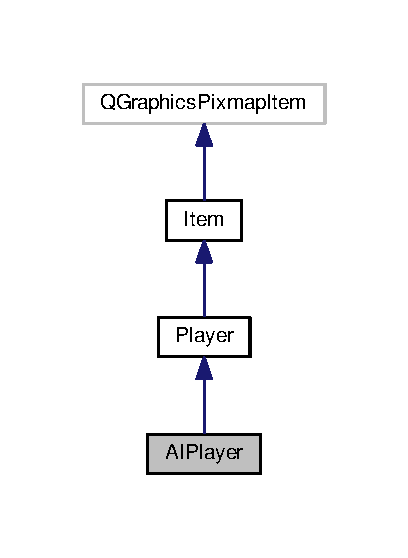
\includegraphics[width=196pt]{class_a_i_player__inherit__graph}
\end{center}
\end{figure}


Collaboration diagram for A\+I\+Player\+:
\nopagebreak
\begin{figure}[H]
\begin{center}
\leavevmode
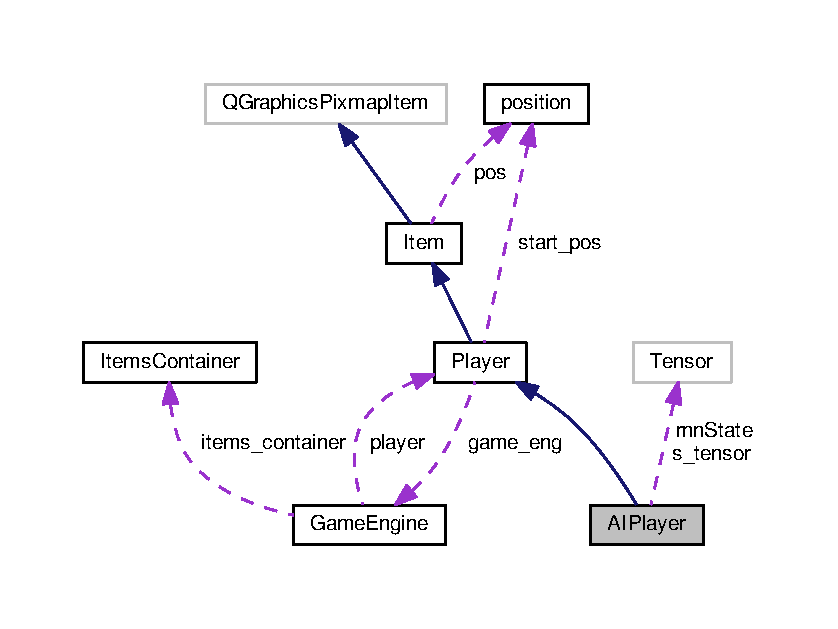
\includegraphics[width=350pt]{class_a_i_player__coll__graph}
\end{center}
\end{figure}
\subsection*{Public Member Functions}
\begin{DoxyCompactItemize}
\item 
{\bfseries A\+I\+Player} (\hyperlink{class_game_engine}{Game\+Engine} $\ast$game\+\_\+eng\+\_\+, const std\+::string \&path)\hypertarget{class_a_i_player_aa75e6656a876ae0d4dc1502754d883ac}{}\label{class_a_i_player_aa75e6656a876ae0d4dc1502754d883ac}

\item 
Tensor \hyperlink{class_a_i_player_ad7462ee157edc5701c3f4534159ab54b}{Predict\+Move} ()
\begin{DoxyCompactList}\small\item\em gets the two most optimal game moves from Q-\/network \end{DoxyCompactList}\item 
virtual void \hyperlink{class_a_i_player_a0a82287b3e1353b58c5dc79d099ab4a6}{Play} ()\hypertarget{class_a_i_player_a0a82287b3e1353b58c5dc79d099ab4a6}{}\label{class_a_i_player_a0a82287b3e1353b58c5dc79d099ab4a6}

\begin{DoxyCompactList}\small\item\em actually plays the game according to Q-\/network predictions \end{DoxyCompactList}\end{DoxyCompactItemize}
\subsection*{Protected Member Functions}
\begin{DoxyCompactItemize}
\item 
Status {\bfseries Load\+Graph} (const string \&graph\+\_\+file\+\_\+name, std\+::unique\+\_\+ptr$<$ tensorflow\+::\+Session $>$ $\ast$session)\hypertarget{class_a_i_player_aac8bd4a862ce36c2baa28ecb363732b4}{}\label{class_a_i_player_aac8bd4a862ce36c2baa28ecb363732b4}

\end{DoxyCompactItemize}
\subsection*{Protected Attributes}
\begin{DoxyCompactItemize}
\item 
Mat {\bfseries state}\hypertarget{class_a_i_player_ab94d1475df2d2902134ccf5b2e9f6741}{}\label{class_a_i_player_ab94d1475df2d2902134ccf5b2e9f6741}

\item 
Tensor {\bfseries s\+\_\+tensor}\hypertarget{class_a_i_player_a273bef59d854a3b944887aef66e916bb}{}\label{class_a_i_player_a273bef59d854a3b944887aef66e916bb}

\item 
std\+::unique\+\_\+ptr$<$ tensorflow\+::\+Session $>$ {\bfseries session}\hypertarget{class_a_i_player_af067956516b244d0f8c3ee01bbbe50b4}{}\label{class_a_i_player_af067956516b244d0f8c3ee01bbbe50b4}

\item 
Tensor {\bfseries rnn\+State}\hypertarget{class_a_i_player_a8480f9a924865fad83075ad453d7ba29}{}\label{class_a_i_player_a8480f9a924865fad83075ad453d7ba29}

\item 
vector$<$ int $>$ {\bfseries recents}\hypertarget{class_a_i_player_addbd2f9dbe9c9956a7b26cbf06f0e53d}{}\label{class_a_i_player_addbd2f9dbe9c9956a7b26cbf06f0e53d}

\item 
vector$<$ bool $>$ {\bfseries moved}\hypertarget{class_a_i_player_a2c2c2cdfbd3ecbcaf564d0c6e1c1f015}{}\label{class_a_i_player_a2c2c2cdfbd3ecbcaf564d0c6e1c1f015}

\end{DoxyCompactItemize}
\subsection*{Additional Inherited Members}


\subsection{Member Function Documentation}
\index{A\+I\+Player@{A\+I\+Player}!Predict\+Move@{Predict\+Move}}
\index{Predict\+Move@{Predict\+Move}!A\+I\+Player@{A\+I\+Player}}
\subsubsection[{\texorpdfstring{Predict\+Move()}{PredictMove()}}]{\setlength{\rightskip}{0pt plus 5cm}Tensor A\+I\+Player\+::\+Predict\+Move (
\begin{DoxyParamCaption}
{}
\end{DoxyParamCaption}
)}\hypertarget{class_a_i_player_ad7462ee157edc5701c3f4534159ab54b}{}\label{class_a_i_player_ad7462ee157edc5701c3f4534159ab54b}


gets the two most optimal game moves from Q-\/network 

\begin{DoxyReturn}{Returns}
tensorflow\+::\+Tensor of size 2x1 
\end{DoxyReturn}


The documentation for this class was generated from the following files\+:\begin{DoxyCompactItemize}
\item 
/home/netsurf/buildspeed/c/src/A\+I\+Player.\+h\item 
/home/netsurf/buildspeed/c/src/A\+I\+Player.\+cpp\end{DoxyCompactItemize}

\hypertarget{class_bonus}{}\section{Bonus Class Reference}
\label{class_bonus}\index{Bonus@{Bonus}}


Inheritance diagram for Bonus\+:\nopagebreak
\begin{figure}[H]
\begin{center}
\leavevmode
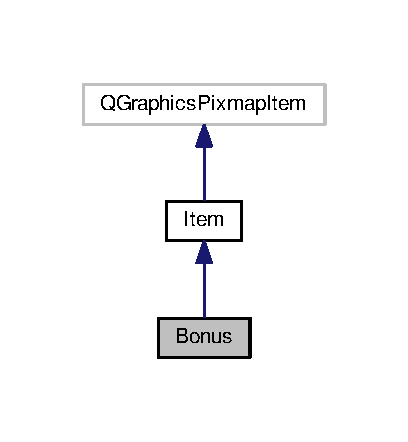
\includegraphics[width=196pt]{class_bonus__inherit__graph}
\end{center}
\end{figure}


Collaboration diagram for Bonus\+:\nopagebreak
\begin{figure}[H]
\begin{center}
\leavevmode
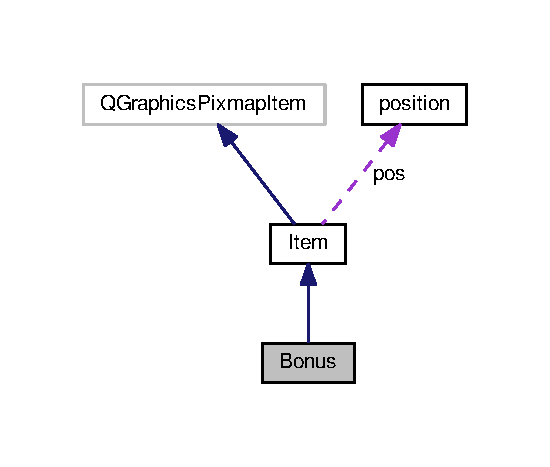
\includegraphics[width=264pt]{class_bonus__coll__graph}
\end{center}
\end{figure}
\subsection*{Public Member Functions}
\begin{DoxyCompactItemize}
\item 
{\bfseries Bonus} (const float intensity\+\_\+, const float reward\+\_\+, const int size\+\_\+)\hypertarget{class_bonus_a151ace5d3747c97287fe7b338f14f3fb}{}\label{class_bonus_a151ace5d3747c97287fe7b338f14f3fb}

\end{DoxyCompactItemize}
\subsection*{Additional Inherited Members}


The documentation for this class was generated from the following files\+:\begin{DoxyCompactItemize}
\item 
/home/netsurf/buildspeed/c/src/Bonus.\+h\item 
/home/netsurf/buildspeed/c/src/Bonus.\+cpp\end{DoxyCompactItemize}

\hypertarget{class_game_engine}{}\section{Game\+Engine Class Reference}
\label{class_game_engine}\index{Game\+Engine@{Game\+Engine}}


Collaboration diagram for Game\+Engine\+:\nopagebreak
\begin{figure}[H]
\begin{center}
\leavevmode
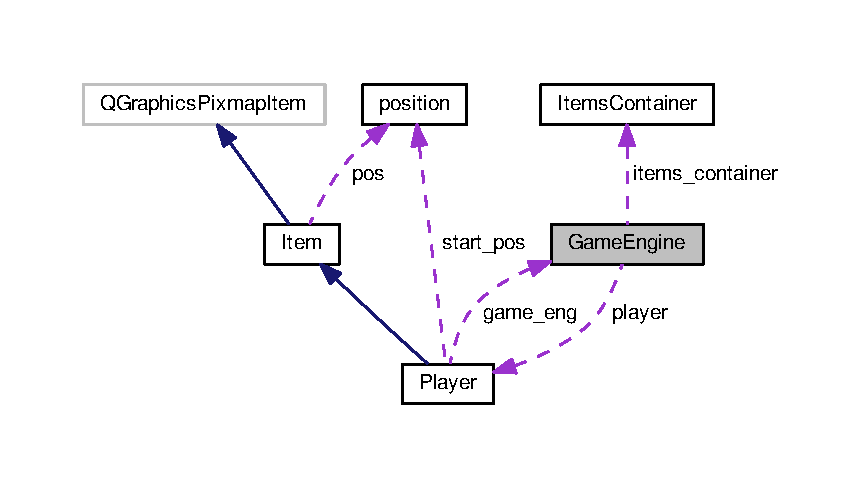
\includegraphics[width=350pt]{class_game_engine__coll__graph}
\end{center}
\end{figure}
\subsection*{Public Member Functions}
\begin{DoxyCompactItemize}
\item 
{\bfseries Game\+Engine} (const int mode\+\_\+, const int sizex, const int sizey)\hypertarget{class_game_engine_afce908a69590e1fbbf5e6c142d8817db}{}\label{class_game_engine_afce908a69590e1fbbf5e6c142d8817db}

\item 
void \hyperlink{class_game_engine_ab7daf2551eca113947559e9f07dae0a7}{Init} ()\hypertarget{class_game_engine_ab7daf2551eca113947559e9f07dae0a7}{}\label{class_game_engine_ab7daf2551eca113947559e9f07dae0a7}

\begin{DoxyCompactList}\small\item\em inits items container with suitable items at random positions \end{DoxyCompactList}\item 
int {\bfseries Get\+Mode} () const \hypertarget{class_game_engine_a7654f7e7c36f08ca30d7ab787b6c8395}{}\label{class_game_engine_a7654f7e7c36f08ca30d7ab787b6c8395}

\item 
int {\bfseries Get\+Round} () const \hypertarget{class_game_engine_a70dbb4a628af69ee9a98bcd0f55cf82b}{}\label{class_game_engine_a70dbb4a628af69ee9a98bcd0f55cf82b}

\item 
int {\bfseries Get\+Score} () const \hypertarget{class_game_engine_aaadf240e3c57133232fbc76a6c7dbef4}{}\label{class_game_engine_aaadf240e3c57133232fbc76a6c7dbef4}

\item 
int {\bfseries Get\+Width} () const \hypertarget{class_game_engine_a8ebfb1997f8ba5e7883eaa5f6dcf07b0}{}\label{class_game_engine_a8ebfb1997f8ba5e7883eaa5f6dcf07b0}

\item 
int {\bfseries Get\+Height} () const \hypertarget{class_game_engine_a6d8b90505d78fed818a60359ece85365}{}\label{class_game_engine_a6d8b90505d78fed818a60359ece85365}

\item 
void \hyperlink{class_game_engine_aafb70dae41903a73df76f638541665f8}{Play} ()\hypertarget{class_game_engine_aafb70dae41903a73df76f638541665f8}{}\label{class_game_engine_aafb70dae41903a73df76f638541665f8}

\begin{DoxyCompactList}\small\item\em calls \hyperlink{class_game_engine_aafb70dae41903a73df76f638541665f8}{Play()} method on current \hyperlink{class_player}{Player} \end{DoxyCompactList}\item 
void \hyperlink{class_game_engine_a7ebc4fbf00f14a405d989ef7c8d8c1c6}{Populate\+Grid} (Q\+Graphics\+Scene $\ast$scene, bool restore=false)
\begin{DoxyCompactList}\small\item\em populates game grid with items from items container \end{DoxyCompactList}\item 
void \hyperlink{class_game_engine_ae831b6dee7c10ddc3cf5bc5d217031b1}{Update} ()\hypertarget{class_game_engine_ae831b6dee7c10ddc3cf5bc5d217031b1}{}\label{class_game_engine_ae831b6dee7c10ddc3cf5bc5d217031b1}

\begin{DoxyCompactList}\small\item\em updates game environment after player\textquotesingle{}s move \end{DoxyCompactList}\item 
void \hyperlink{class_game_engine_ac3a1cfe6f6278619a1158dad566cd87c}{To\+Matrix} (vector$<$ cv\+::\+Mat $>$ \&matrix)\hypertarget{class_game_engine_ac3a1cfe6f6278619a1158dad566cd87c}{}\label{class_game_engine_ac3a1cfe6f6278619a1158dad566cd87c}

\begin{DoxyCompactList}\small\item\em exports current game state as a Open\+CV matrix \end{DoxyCompactList}\item 
\hyperlink{structposition}{position} \hyperlink{class_game_engine_abd94740b8a8ac3bf474cf695023473ed}{Pick\+New\+Position} ()\hypertarget{class_game_engine_abd94740b8a8ac3bf474cf695023473ed}{}\label{class_game_engine_abd94740b8a8ac3bf474cf695023473ed}

\begin{DoxyCompactList}\small\item\em returns an empty position on the grid \end{DoxyCompactList}\item 
void \hyperlink{class_game_engine_ab6a4193dd629e968bdc3ea8eae259b13}{Set\+Player\+Tooltip\+Text} (const Q\+String str)\hypertarget{class_game_engine_ab6a4193dd629e968bdc3ea8eae259b13}{}\label{class_game_engine_ab6a4193dd629e968bdc3ea8eae259b13}

\begin{DoxyCompactList}\small\item\em updates current player\textquotesingle{}s score tooltip \end{DoxyCompactList}\end{DoxyCompactItemize}
\subsection*{Protected Attributes}
\begin{DoxyCompactItemize}
\item 
int {\bfseries round}\hypertarget{class_game_engine_aa28d21ca6308c68892642f112a9f576a}{}\label{class_game_engine_aa28d21ca6308c68892642f112a9f576a}

\item 
int {\bfseries mode}\hypertarget{class_game_engine_a7145ec824cc63e5323fd8f5a074ec342}{}\label{class_game_engine_a7145ec824cc63e5323fd8f5a074ec342}

\item 
int {\bfseries sizeX}\hypertarget{class_game_engine_a5b500d38dc898994a2e0f53a923fe0a5}{}\label{class_game_engine_a5b500d38dc898994a2e0f53a923fe0a5}

\item 
int {\bfseries sizeY}\hypertarget{class_game_engine_ad720d519a87110aea56f8c896de586e9}{}\label{class_game_engine_ad720d519a87110aea56f8c896de586e9}

\item 
\hyperlink{class_items_container}{Items\+Container} {\bfseries items\+\_\+container}\hypertarget{class_game_engine_a306792ba7de2bd02ac487425a449992c}{}\label{class_game_engine_a306792ba7de2bd02ac487425a449992c}

\item 
\hyperlink{class_player}{Player} $\ast$ {\bfseries player} = nullptr\hypertarget{class_game_engine_aabcb1d42f2f2a0d49abb6f010599eb78}{}\label{class_game_engine_aabcb1d42f2f2a0d49abb6f010599eb78}

\item 
Q\+Sound\+Effect {\bfseries bonus\+\_\+sound}\hypertarget{class_game_engine_a5e986b659dd5a4c57039332c7e468e99}{}\label{class_game_engine_a5e986b659dd5a4c57039332c7e468e99}

\item 
Q\+Sound\+Effect {\bfseries hole\+\_\+sound}\hypertarget{class_game_engine_a218635f0033570563613c93a94decdf6}{}\label{class_game_engine_a218635f0033570563613c93a94decdf6}

\end{DoxyCompactItemize}


\subsection{Member Function Documentation}
\index{Game\+Engine@{Game\+Engine}!Populate\+Grid@{Populate\+Grid}}
\index{Populate\+Grid@{Populate\+Grid}!Game\+Engine@{Game\+Engine}}
\subsubsection[{\texorpdfstring{Populate\+Grid(\+Q\+Graphics\+Scene $\ast$scene, bool restore=false)}{PopulateGrid(QGraphicsScene *scene, bool restore=false)}}]{\setlength{\rightskip}{0pt plus 5cm}void Game\+Engine\+::\+Populate\+Grid (
\begin{DoxyParamCaption}
\item[{Q\+Graphics\+Scene $\ast$}]{scene, }
\item[{bool}]{restore = {\ttfamily false}}
\end{DoxyParamCaption}
)}\hypertarget{class_game_engine_a7ebc4fbf00f14a405d989ef7c8d8c1c6}{}\label{class_game_engine_a7ebc4fbf00f14a405d989ef7c8d8c1c6}


populates game grid with items from items container 


\begin{DoxyParams}{Parameters}
{\em scene} & is the game grid, restore is true if grid items backup has to be restored \\
\hline
\end{DoxyParams}


The documentation for this class was generated from the following files\+:\begin{DoxyCompactItemize}
\item 
/home/netsurf/buildspeed/c/src/Game\+Engine.\+h\item 
/home/netsurf/buildspeed/c/src/Game\+Engine.\+cpp\end{DoxyCompactItemize}

\hypertarget{class_game_view}{}\section{Game\+View Class Reference}
\label{class_game_view}\index{Game\+View@{Game\+View}}


Inheritance diagram for Game\+View\+:\nopagebreak
\begin{figure}[H]
\begin{center}
\leavevmode
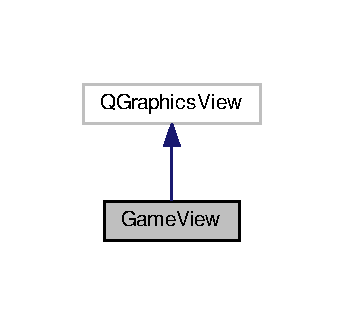
\includegraphics[width=165pt]{class_game_view__inherit__graph}
\end{center}
\end{figure}


Collaboration diagram for Game\+View\+:\nopagebreak
\begin{figure}[H]
\begin{center}
\leavevmode
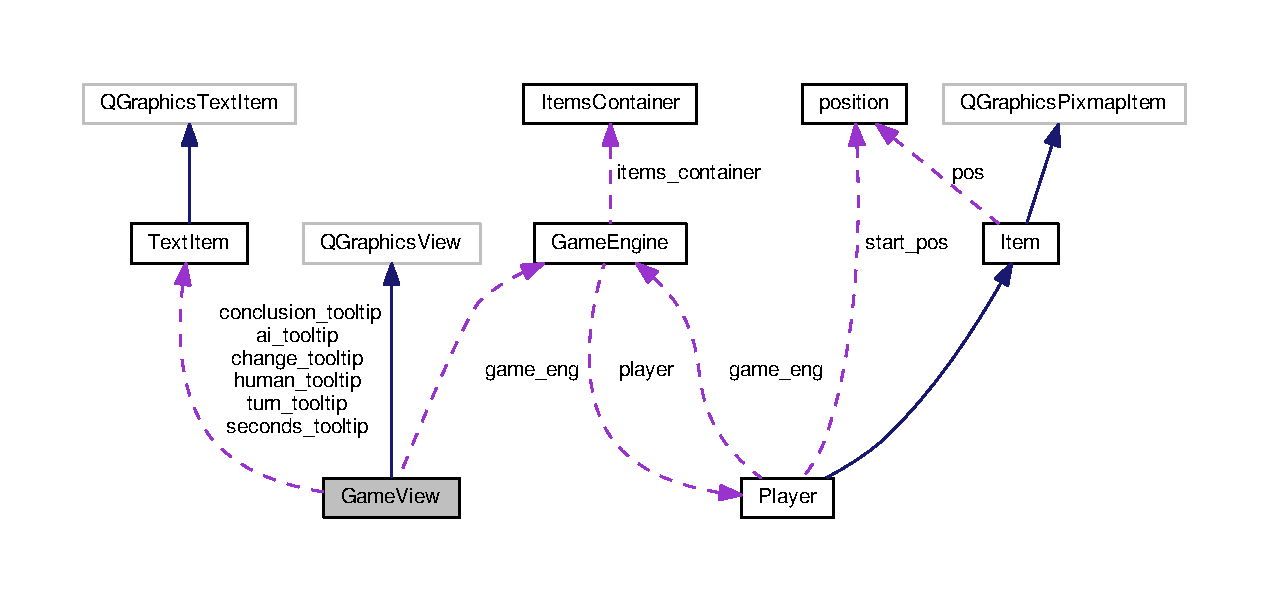
\includegraphics[width=350pt]{class_game_view__coll__graph}
\end{center}
\end{figure}
\subsection*{Public Member Functions}
\begin{DoxyCompactItemize}
\item 
{\bfseries Game\+View} (const int mode\+\_\+, Q\+Widget $\ast$parent=0)\hypertarget{class_game_view_a10ff55ad9e283fc42d4a1eecfe6ee2d8}{}\label{class_game_view_a10ff55ad9e283fc42d4a1eecfe6ee2d8}

\item 
void \hyperlink{class_game_view_ab44f4473d1292b3e67bff57cf04138d7}{Set\+Path} (const std\+::string path\+\_\+)
\begin{DoxyCompactList}\small\item\em stores working directory \end{DoxyCompactList}\item 
std\+::string {\bfseries Get\+Path} ()\hypertarget{class_game_view_a26dcec76a5c6778b4f61c972e1675089}{}\label{class_game_view_a26dcec76a5c6778b4f61c972e1675089}

\item 
void \hyperlink{class_game_view_a61fff3c00a8b13002e3b0efffb1e9ad0}{Pass\+To\+AI} ()\hypertarget{class_game_view_a61fff3c00a8b13002e3b0efffb1e9ad0}{}\label{class_game_view_a61fff3c00a8b13002e3b0efffb1e9ad0}

\begin{DoxyCompactList}\small\item\em resets the game environment in order to let AI agent play \end{DoxyCompactList}\item 
void {\bfseries key\+Press\+Event} (Q\+Key\+Event $\ast$event)\hypertarget{class_game_view_ab8244fb1cf987e1eb91d62968b3d2cfd}{}\label{class_game_view_ab8244fb1cf987e1eb91d62968b3d2cfd}

\item 
void \hyperlink{class_game_view_a7d840226c0e3d25380081cede750ce5b}{Flash\+Score\+Change} (const float delta)
\begin{DoxyCompactList}\small\item\em displays score change as consequence of a move \end{DoxyCompactList}\item 
void \hyperlink{class_game_view_adf946f732dca534a0af220d728fd1a22}{Set\+Player\+Tooltip\+Text} (const Q\+String str)
\begin{DoxyCompactList}\small\item\em displays score change as consequence of a move \end{DoxyCompactList}\end{DoxyCompactItemize}
\subsection*{Static Public Attributes}
\begin{DoxyCompactItemize}
\item 
static const int {\bfseries rect\+\_\+margin} = 20\hypertarget{class_game_view_a7044d555439ae4b05b2d06c2ee63d294}{}\label{class_game_view_a7044d555439ae4b05b2d06c2ee63d294}

\item 
static const int {\bfseries seconds\+\_\+turn} = 15\hypertarget{class_game_view_a5fc396e1ec2179e006f4e6dd0f9915cb}{}\label{class_game_view_a5fc396e1ec2179e006f4e6dd0f9915cb}

\end{DoxyCompactItemize}
\subsection*{Protected Member Functions}
\begin{DoxyCompactItemize}
\item 
void {\bfseries Restore\+Grid} ()\hypertarget{class_game_view_a6e52f2706160a781da99bdeb5a2a6082}{}\label{class_game_view_a6e52f2706160a781da99bdeb5a2a6082}

\item 
void {\bfseries Reset\+Timer} ()\hypertarget{class_game_view_af23e016497d307afd3b8eebd41086de0}{}\label{class_game_view_af23e016497d307afd3b8eebd41086de0}

\item 
void {\bfseries Play\+Again} ()\hypertarget{class_game_view_a53c1f97294b6be0e41cc627fc21abd5d}{}\label{class_game_view_a53c1f97294b6be0e41cc627fc21abd5d}

\end{DoxyCompactItemize}
\subsection*{Protected Attributes}
\begin{DoxyCompactItemize}
\item 
\hyperlink{class_text_item}{Text\+Item} $\ast$ {\bfseries turn\+\_\+tooltip} = nullptr\hypertarget{class_game_view_ad2bffcf684b7e40e9253b803f7e551e3}{}\label{class_game_view_ad2bffcf684b7e40e9253b803f7e551e3}

\item 
\hyperlink{class_text_item}{Text\+Item} $\ast$ {\bfseries human\+\_\+tooltip} = nullptr\hypertarget{class_game_view_a94384f3324a363d01a6a032fcc5343d3}{}\label{class_game_view_a94384f3324a363d01a6a032fcc5343d3}

\item 
\hyperlink{class_text_item}{Text\+Item} $\ast$ {\bfseries ai\+\_\+tooltip} = nullptr\hypertarget{class_game_view_a91eca658fe5c578738ac3df698b2c764}{}\label{class_game_view_a91eca658fe5c578738ac3df698b2c764}

\item 
\hyperlink{class_text_item}{Text\+Item} $\ast$ {\bfseries conclusion\+\_\+tooltip} = nullptr\hypertarget{class_game_view_a2594d4271aa9afcde50aab83ef78f385}{}\label{class_game_view_a2594d4271aa9afcde50aab83ef78f385}

\item 
\hyperlink{class_text_item}{Text\+Item} $\ast$ {\bfseries change\+\_\+tooltip} = nullptr\hypertarget{class_game_view_a9f2dcc56b12ec541b5a7882ec1abb2e7}{}\label{class_game_view_a9f2dcc56b12ec541b5a7882ec1abb2e7}

\item 
\hyperlink{class_text_item}{Text\+Item} $\ast$ {\bfseries seconds\+\_\+tooltip} = nullptr\hypertarget{class_game_view_a28bfa10f16a992c83d36994c334e208c}{}\label{class_game_view_a28bfa10f16a992c83d36994c334e208c}

\item 
string {\bfseries path}\hypertarget{class_game_view_a396325f196775191890d3262ecb5e9ff}{}\label{class_game_view_a396325f196775191890d3262ecb5e9ff}

\item 
Q\+Graphics\+Scene $\ast$ {\bfseries scene} = nullptr\hypertarget{class_game_view_aa96ff0163839f95478ed0de98d3e4e51}{}\label{class_game_view_aa96ff0163839f95478ed0de98d3e4e51}

\item 
\hyperlink{class_game_engine}{Game\+Engine} {\bfseries game\+\_\+eng}\hypertarget{class_game_view_a1f53dd762f200a230c3b90510c14a30a}{}\label{class_game_view_a1f53dd762f200a230c3b90510c14a30a}

\item 
Q\+Timer $\ast$ {\bfseries timer}\hypertarget{class_game_view_ab651668a749d0a823b67b5b260be2125}{}\label{class_game_view_ab651668a749d0a823b67b5b260be2125}

\item 
int {\bfseries seconds}\hypertarget{class_game_view_a005c0fe1f5c3b898ae4ec7ee4496ebab}{}\label{class_game_view_a005c0fe1f5c3b898ae4ec7ee4496ebab}

\end{DoxyCompactItemize}
\subsection*{Static Protected Attributes}
\begin{DoxyCompactItemize}
\item 
static const Q\+String {\bfseries human\+\_\+turn} = \char`\"{}$<$h1$>$It\textquotesingle{}s human turn.$<$/h1$>$\char`\"{}\hypertarget{class_game_view_a8d393d08a1b5e348fc36d848fb9e590b}{}\label{class_game_view_a8d393d08a1b5e348fc36d848fb9e590b}

\item 
static const Q\+String {\bfseries ai\+\_\+turn} = \char`\"{}$<$h1$>$Now it\textquotesingle{}s AI turn...$<$/h1$>$\char`\"{}\hypertarget{class_game_view_a4a605ac7010042321724e49c4a43a485}{}\label{class_game_view_a4a605ac7010042321724e49c4a43a485}

\item 
static const Q\+String {\bfseries initial\+\_\+human\+\_\+score\+\_\+tooltip} = \char`\"{}Human score\+: $<$b style=\textquotesingle{}color\+:\#06\+C; font-\/size\+:20px;\textquotesingle{}$>$0$<$/b$>$, Moves\+:$<$b$>$0/50$<$/b$>$\char`\"{}\hypertarget{class_game_view_a0575767749bddb4f4552bc73caa1f2bd}{}\label{class_game_view_a0575767749bddb4f4552bc73caa1f2bd}

\item 
static const Q\+String {\bfseries initial\+\_\+ai\+\_\+score\+\_\+tooltip} = \char`\"{}AI score\+: $<$b style=\textquotesingle{}color\+:\#06\+C; font-\/size\+:20px;\textquotesingle{}$>$0$<$/b$>$, Moves\+:$<$b$>$0/50$<$/b$>$\char`\"{}\hypertarget{class_game_view_a9503edee1bdd2d5acf8c42d368392b94}{}\label{class_game_view_a9503edee1bdd2d5acf8c42d368392b94}

\item 
static const string {\bfseries seconds\+\_\+tooltip\+\_\+text} =\char`\"{}$<$h1 style=\textquotesingle{}color\+:red\textquotesingle{}$>$\%1\% seconds$<$/h1$>$\char`\"{}\hypertarget{class_game_view_a0875a9ee7af2bf612ee3d0e01bdc4683}{}\label{class_game_view_a0875a9ee7af2bf612ee3d0e01bdc4683}

\item 
static const string {\bfseries score\+\_\+change\+\_\+positive\+\_\+text} =\char`\"{}$<$h1 style=\textquotesingle{}color\+:green;\textquotesingle{}$>$+\%1\%$<$/h1$>$\char`\"{}\hypertarget{class_game_view_a119becaa2deb77dacd5b1e3385c49b2d}{}\label{class_game_view_a119becaa2deb77dacd5b1e3385c49b2d}

\item 
static const string {\bfseries score\+\_\+change\+\_\+negative\+\_\+text} =\char`\"{}$<$h1 style=\textquotesingle{}color\+:red;\textquotesingle{}$>$\%1\%$<$/h1$>$\char`\"{}\hypertarget{class_game_view_a199fa1bbcc63fb0890bbddf6cfa6ba54}{}\label{class_game_view_a199fa1bbcc63fb0890bbddf6cfa6ba54}

\end{DoxyCompactItemize}


\subsection{Member Function Documentation}
\index{Game\+View@{Game\+View}!Flash\+Score\+Change@{Flash\+Score\+Change}}
\index{Flash\+Score\+Change@{Flash\+Score\+Change}!Game\+View@{Game\+View}}
\subsubsection[{\texorpdfstring{Flash\+Score\+Change(const float delta)}{FlashScoreChange(const float delta)}}]{\setlength{\rightskip}{0pt plus 5cm}void Game\+View\+::\+Flash\+Score\+Change (
\begin{DoxyParamCaption}
\item[{const float}]{delta}
\end{DoxyParamCaption}
)}\hypertarget{class_game_view_a7d840226c0e3d25380081cede750ce5b}{}\label{class_game_view_a7d840226c0e3d25380081cede750ce5b}


displays score change as consequence of a move 


\begin{DoxyParams}{Parameters}
{\em delta} & is the score variation \\
\hline
\end{DoxyParams}
\index{Game\+View@{Game\+View}!Set\+Path@{Set\+Path}}
\index{Set\+Path@{Set\+Path}!Game\+View@{Game\+View}}
\subsubsection[{\texorpdfstring{Set\+Path(const std\+::string path\+\_\+)}{SetPath(const std::string path_)}}]{\setlength{\rightskip}{0pt plus 5cm}void Game\+View\+::\+Set\+Path (
\begin{DoxyParamCaption}
\item[{const std\+::string}]{path\+\_\+}
\end{DoxyParamCaption}
)\hspace{0.3cm}{\ttfamily [inline]}}\hypertarget{class_game_view_ab44f4473d1292b3e67bff57cf04138d7}{}\label{class_game_view_ab44f4473d1292b3e67bff57cf04138d7}


stores working directory 


\begin{DoxyParams}{Parameters}
{\em path} & is the working directory path \\
\hline
\end{DoxyParams}
\index{Game\+View@{Game\+View}!Set\+Player\+Tooltip\+Text@{Set\+Player\+Tooltip\+Text}}
\index{Set\+Player\+Tooltip\+Text@{Set\+Player\+Tooltip\+Text}!Game\+View@{Game\+View}}
\subsubsection[{\texorpdfstring{Set\+Player\+Tooltip\+Text(const Q\+String str)}{SetPlayerTooltipText(const QString str)}}]{\setlength{\rightskip}{0pt plus 5cm}void Game\+View\+::\+Set\+Player\+Tooltip\+Text (
\begin{DoxyParamCaption}
\item[{const Q\+String}]{str}
\end{DoxyParamCaption}
)}\hypertarget{class_game_view_adf946f732dca534a0af220d728fd1a22}{}\label{class_game_view_adf946f732dca534a0af220d728fd1a22}


displays score change as consequence of a move 


\begin{DoxyParams}{Parameters}
{\em delta} & is the score variation \\
\hline
\end{DoxyParams}


The documentation for this class was generated from the following files\+:\begin{DoxyCompactItemize}
\item 
/home/netsurf/buildspeed/c/src/Game\+View.\+h\item 
/home/netsurf/buildspeed/c/src/Game\+View.\+cpp\end{DoxyCompactItemize}

\hypertarget{class_hole}{}\section{Hole Class Reference}
\label{class_hole}\index{Hole@{Hole}}


Inheritance diagram for Hole\+:
\nopagebreak
\begin{figure}[H]
\begin{center}
\leavevmode
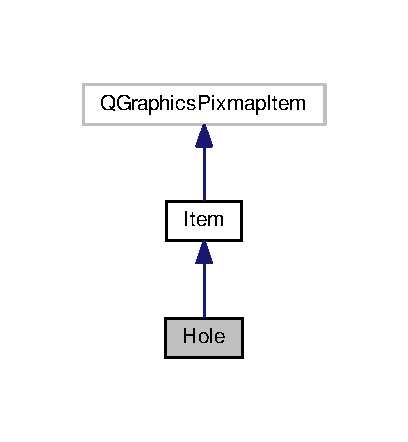
\includegraphics[width=196pt]{class_hole__inherit__graph}
\end{center}
\end{figure}


Collaboration diagram for Hole\+:
\nopagebreak
\begin{figure}[H]
\begin{center}
\leavevmode
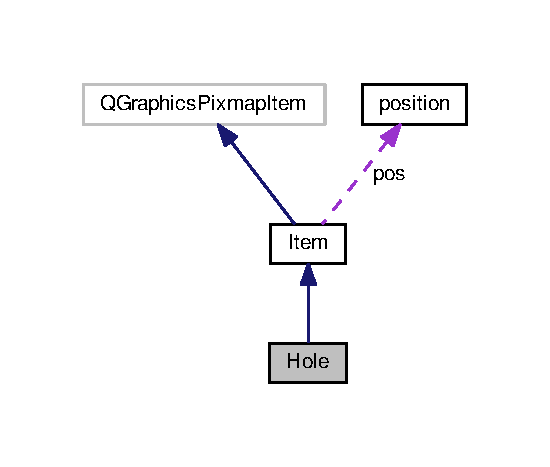
\includegraphics[width=264pt]{class_hole__coll__graph}
\end{center}
\end{figure}
\subsection*{Public Member Functions}
\begin{DoxyCompactItemize}
\item 
{\bfseries Hole} (const float intensity\+\_\+, const float reward\+\_\+)\hypertarget{class_hole_abe1a64c7a1c55a7da8fd489d02ea2bc8}{}\label{class_hole_abe1a64c7a1c55a7da8fd489d02ea2bc8}

\end{DoxyCompactItemize}
\subsection*{Additional Inherited Members}


The documentation for this class was generated from the following files\+:\begin{DoxyCompactItemize}
\item 
/home/netsurf/buildspeed/c/src/Hole.\+h\item 
/home/netsurf/buildspeed/c/src/Hole.\+cpp\end{DoxyCompactItemize}

\hypertarget{class_human_player}{}\section{Human\+Player Class Reference}
\label{class_human_player}\index{Human\+Player@{Human\+Player}}


Inheritance diagram for Human\+Player\+:\nopagebreak
\begin{figure}[H]
\begin{center}
\leavevmode
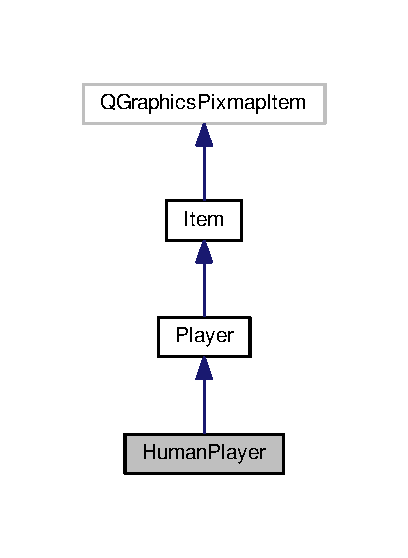
\includegraphics[width=196pt]{class_human_player__inherit__graph}
\end{center}
\end{figure}


Collaboration diagram for Human\+Player\+:\nopagebreak
\begin{figure}[H]
\begin{center}
\leavevmode
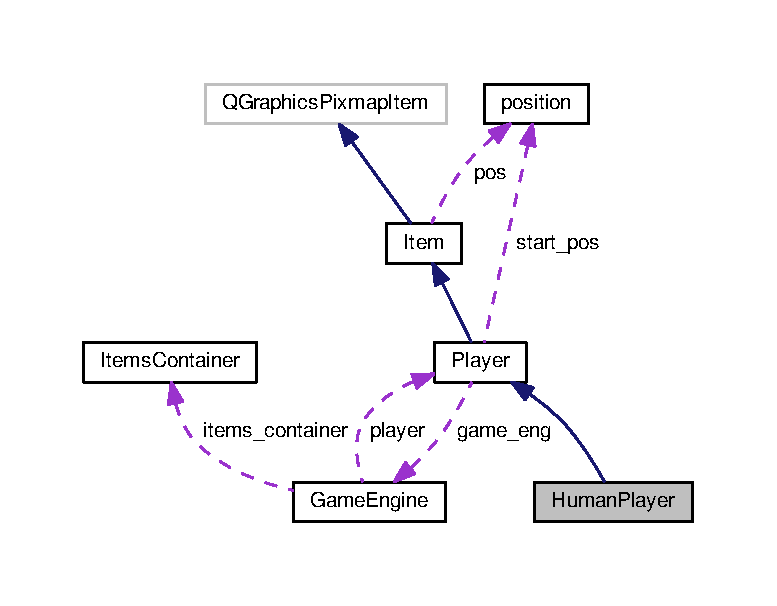
\includegraphics[width=350pt]{class_human_player__coll__graph}
\end{center}
\end{figure}
\subsection*{Public Member Functions}
\begin{DoxyCompactItemize}
\item 
{\bfseries Human\+Player} (\hyperlink{class_game_engine}{Game\+Engine} $\ast$game\+\_\+eng\+\_\+)\hypertarget{class_human_player_a8c9446abf36e24e405d580928151bc50}{}\label{class_human_player_a8c9446abf36e24e405d580928151bc50}

\item 
virtual void \hyperlink{class_human_player_aefcbcec78412bcc9d46a39324f9f2263}{Play} ()\hypertarget{class_human_player_aefcbcec78412bcc9d46a39324f9f2263}{}\label{class_human_player_aefcbcec78412bcc9d46a39324f9f2263}

\begin{DoxyCompactList}\small\item\em prepares the item for playing (focuses the item and backups start position) \end{DoxyCompactList}\item 
void \hyperlink{class_human_player_aef6252dc1b716e9bf5e4da125f811b98}{key\+Press\+Event} (Q\+Key\+Event $\ast$event)
\begin{DoxyCompactList}\small\item\em moves the player if arrow keys are pressed \end{DoxyCompactList}\item 
void {\bfseries key\+Release\+Event} (Q\+Key\+Event $\ast$event)\hypertarget{class_human_player_a58a146dcbb5345557d5224fdabd336dc}{}\label{class_human_player_a58a146dcbb5345557d5224fdabd336dc}

\end{DoxyCompactItemize}
\subsection*{Protected Attributes}
\begin{DoxyCompactItemize}
\item 
Q\+Set$<$ int $>$ {\bfseries keys\+Pressed}\hypertarget{class_human_player_a15509afba818f1d43397ee1223362e3a}{}\label{class_human_player_a15509afba818f1d43397ee1223362e3a}

\end{DoxyCompactItemize}
\subsection*{Additional Inherited Members}


\subsection{Member Function Documentation}
\index{Human\+Player@{Human\+Player}!key\+Press\+Event@{key\+Press\+Event}}
\index{key\+Press\+Event@{key\+Press\+Event}!Human\+Player@{Human\+Player}}
\subsubsection[{\texorpdfstring{key\+Press\+Event(\+Q\+Key\+Event $\ast$event)}{keyPressEvent(QKeyEvent *event)}}]{\setlength{\rightskip}{0pt plus 5cm}void Human\+Player\+::key\+Press\+Event (
\begin{DoxyParamCaption}
\item[{Q\+Key\+Event $\ast$}]{event}
\end{DoxyParamCaption}
)}\hypertarget{class_human_player_aef6252dc1b716e9bf5e4da125f811b98}{}\label{class_human_player_aef6252dc1b716e9bf5e4da125f811b98}


moves the player if arrow keys are pressed 


\begin{DoxyParams}{Parameters}
{\em event} & describes the key pressed \\
\hline
\end{DoxyParams}


The documentation for this class was generated from the following files\+:\begin{DoxyCompactItemize}
\item 
/home/netsurf/buildspeed/c/src/Human\+Player.\+h\item 
/home/netsurf/buildspeed/c/src/Human\+Player.\+cpp\end{DoxyCompactItemize}

\hypertarget{class_item}{}\section{Item Class Reference}
\label{class_item}\index{Item@{Item}}


The \hyperlink{class_item}{Item} class represents any pickable item the player can run into.  




{\ttfamily \#include $<$Item.\+h$>$}



Inheritance diagram for Item\+:\nopagebreak
\begin{figure}[H]
\begin{center}
\leavevmode
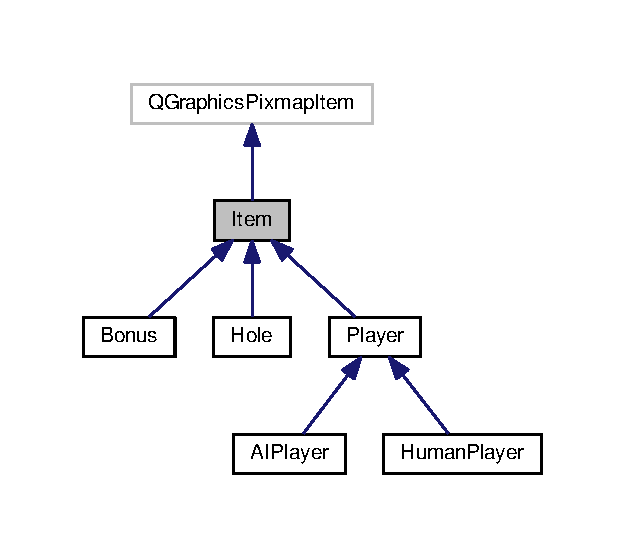
\includegraphics[width=300pt]{class_item__inherit__graph}
\end{center}
\end{figure}


Collaboration diagram for Item\+:\nopagebreak
\begin{figure}[H]
\begin{center}
\leavevmode
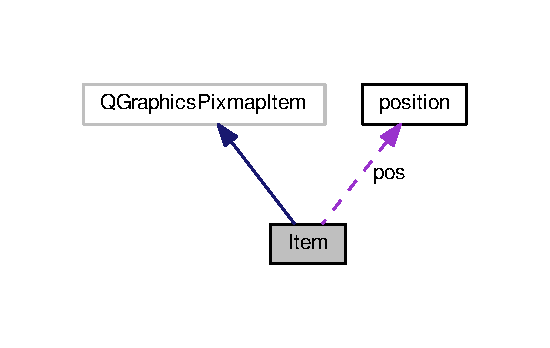
\includegraphics[width=264pt]{class_item__coll__graph}
\end{center}
\end{figure}
\subsection*{Public Member Functions}
\begin{DoxyCompactItemize}
\item 
{\bfseries Item} (Q\+Pixmap pixmap, const int count\+\_\+=0, const int type\+\_\+=Item\+::\+B\+OY, const float intensity\+\_\+=1, const float reward\+\_\+=0)\hypertarget{class_item_a8560c460d411e02eaf1c895927d87e2c}{}\label{class_item_a8560c460d411e02eaf1c895927d87e2c}

\item 
void {\bfseries set\+Pos\+Index} (const int sx, const int sy)\hypertarget{class_item_a705067b62641b477184ed230dfe73636}{}\label{class_item_a705067b62641b477184ed230dfe73636}

\item 
void {\bfseries Set\+Position} (const \hyperlink{structposition}{position} pos\+\_\+)\hypertarget{class_item_a8eae93e3528474efa4b3921e9c11b006}{}\label{class_item_a8eae93e3528474efa4b3921e9c11b006}

\item 
\hyperlink{structposition}{position} {\bfseries Get\+Position} ()\hypertarget{class_item_a6d1dcc0c0328d362061bb1a435935348}{}\label{class_item_a6d1dcc0c0328d362061bb1a435935348}

\item 
float {\bfseries Get\+Intensity} ()\hypertarget{class_item_ab1201c61f4120622de9443ca9bbce176}{}\label{class_item_ab1201c61f4120622de9443ca9bbce176}

\item 
int {\bfseries Get\+Type} ()\hypertarget{class_item_aa6867231a1219d677855c79eaeb558e6}{}\label{class_item_aa6867231a1219d677855c79eaeb558e6}

\item 
float {\bfseries Get\+Reward} ()\hypertarget{class_item_a11882ba846bcdd009607f4660afdb59b}{}\label{class_item_a11882ba846bcdd009607f4660afdb59b}

\item 
void {\bfseries Refresh\+Position} ()\hypertarget{class_item_a6afc8b5c805e0fd3655468f3609a4eb1}{}\label{class_item_a6afc8b5c805e0fd3655468f3609a4eb1}

\end{DoxyCompactItemize}
\subsection*{Static Public Attributes}
\begin{DoxyCompactItemize}
\item 
static const int {\bfseries B\+OY} = 2\hypertarget{class_item_a70873a5ab783160390c311623837b5a5}{}\label{class_item_a70873a5ab783160390c311623837b5a5}

\item 
static const int {\bfseries H\+O\+LE} =0\hypertarget{class_item_abd114fce352b909292f0cf6dc89b4487}{}\label{class_item_abd114fce352b909292f0cf6dc89b4487}

\item 
static const int {\bfseries B\+O\+N\+US} = 1\hypertarget{class_item_a76b7a450081315e261c475736dfb74a3}{}\label{class_item_a76b7a450081315e261c475736dfb74a3}

\end{DoxyCompactItemize}
\subsection*{Protected Attributes}
\begin{DoxyCompactItemize}
\item 
Q\+Graphics\+Text\+Item $\ast$ {\bfseries count\+\_\+text}\hypertarget{class_item_ae17075ec9a03088db6f561c4f9c76742}{}\label{class_item_ae17075ec9a03088db6f561c4f9c76742}

\item 
float {\bfseries intensity}\hypertarget{class_item_a27b5db0436c59d6c8f91c3bc787bf793}{}\label{class_item_a27b5db0436c59d6c8f91c3bc787bf793}

\item 
int {\bfseries type}\hypertarget{class_item_a22a98aed7ce8f0314b597a5739c415b7}{}\label{class_item_a22a98aed7ce8f0314b597a5739c415b7}

\item 
float {\bfseries reward}\hypertarget{class_item_a96e9e465bc41c9b5b775281771019587}{}\label{class_item_a96e9e465bc41c9b5b775281771019587}

\item 
\hyperlink{structposition}{position} {\bfseries pos}\hypertarget{class_item_a7ec0bf2287ce0cba665689292a86e429}{}\label{class_item_a7ec0bf2287ce0cba665689292a86e429}

\end{DoxyCompactItemize}


\subsection{Detailed Description}
The \hyperlink{class_item}{Item} class represents any pickable item the player can run into. 

The documentation for this class was generated from the following files\+:\begin{DoxyCompactItemize}
\item 
/home/netsurf/buildspeed/c/src/Item.\+h\item 
/home/netsurf/buildspeed/c/src/Item.\+cpp\end{DoxyCompactItemize}

\hypertarget{class_items_container}{}\section{Items\+Container Class Reference}
\label{class_items_container}\index{Items\+Container@{Items\+Container}}
\subsection*{Classes}
\begin{DoxyCompactItemize}
\item 
class \hyperlink{class_items_container_1_1_iterator}{Iterator}
\end{DoxyCompactItemize}
\subsection*{Public Member Functions}
\begin{DoxyCompactItemize}
\item 
void {\bfseries Create\+Item} (const float intensity, const int type, const float reward, const \hyperlink{structposition}{position} pos, int size=0)\hypertarget{class_items_container_a20a17dd5ea76284f08058dcef2ed2ae1}{}\label{class_items_container_a20a17dd5ea76284f08058dcef2ed2ae1}

\item 
void {\bfseries Backup} ()\hypertarget{class_items_container_ac5fda56d21cb3dbfe3539324676d78b4}{}\label{class_items_container_ac5fda56d21cb3dbfe3539324676d78b4}

\item 
void {\bfseries Restore\+Backup} ()\hypertarget{class_items_container_ae8da03f9a1092503250d7cc3945c3110}{}\label{class_items_container_ae8da03f9a1092503250d7cc3945c3110}

\item 
void {\bfseries Clear} ()\hypertarget{class_items_container_afe3c71e5ab8edfb9cc51d0ea2046813d}{}\label{class_items_container_afe3c71e5ab8edfb9cc51d0ea2046813d}

\end{DoxyCompactItemize}
\subsection*{Protected Attributes}
\begin{DoxyCompactItemize}
\item 
std\+::vector$<$ \hyperlink{class_item}{Item} $\ast$ $>$ {\bfseries objects}\hypertarget{class_items_container_affafed4ab97909cb54474eb7cbab2847}{}\label{class_items_container_affafed4ab97909cb54474eb7cbab2847}

\item 
std\+::vector$<$ \hyperlink{structposition}{position} $>$ {\bfseries start\+\_\+positions}\hypertarget{class_items_container_a423e6fe91a727429743660295c849f1f}{}\label{class_items_container_a423e6fe91a727429743660295c849f1f}

\end{DoxyCompactItemize}
\subsection*{Friends}
\begin{DoxyCompactItemize}
\item 
class {\bfseries Iterator}\hypertarget{class_items_container_a9830fc407400559db7e7783cc10a9394}{}\label{class_items_container_a9830fc407400559db7e7783cc10a9394}

\end{DoxyCompactItemize}


The documentation for this class was generated from the following files\+:\begin{DoxyCompactItemize}
\item 
/home/netsurf/buildspeed/c/src/Items\+Container.\+h\item 
/home/netsurf/buildspeed/c/src/Items\+Container.\+cpp\end{DoxyCompactItemize}

\hypertarget{class_items_container_1_1_iterator}{}\section{Items\+Container\+:\+:Iterator Class Reference}
\label{class_items_container_1_1_iterator}\index{Items\+Container\+::\+Iterator@{Items\+Container\+::\+Iterator}}
\subsection*{Public Member Functions}
\begin{DoxyCompactItemize}
\item 
{\bfseries Iterator} (\hyperlink{class_items_container}{Items\+Container} \&container\+\_\+)\hypertarget{class_items_container_1_1_iterator_a6874740b122450e322ac35b6b3f556ed}{}\label{class_items_container_1_1_iterator_a6874740b122450e322ac35b6b3f556ed}

\item 
void {\bfseries Reset} ()\hypertarget{class_items_container_1_1_iterator_aa2d6f31b2a31c3a52923e475813a24b2}{}\label{class_items_container_1_1_iterator_aa2d6f31b2a31c3a52923e475813a24b2}

\item 
\hyperlink{class_item}{Item} $\ast$ {\bfseries Get\+Next} ()\hypertarget{class_items_container_1_1_iterator_a33e4c357fcf13b1aaaa88fbe4dbab294}{}\label{class_items_container_1_1_iterator_a33e4c357fcf13b1aaaa88fbe4dbab294}

\item 
bool {\bfseries Has\+Next} () const \hypertarget{class_items_container_1_1_iterator_a57ccfac6e90ecc00700fb8f1127ecec2}{}\label{class_items_container_1_1_iterator_a57ccfac6e90ecc00700fb8f1127ecec2}

\end{DoxyCompactItemize}


The documentation for this class was generated from the following file\+:\begin{DoxyCompactItemize}
\item 
/home/netsurf/buildspeed/c/src/Items\+Container.\+h\end{DoxyCompactItemize}

\hypertarget{class_main_screen}{}\section{Main\+Screen Class Reference}
\label{class_main_screen}\index{Main\+Screen@{Main\+Screen}}


The \hyperlink{class_main_screen}{Main\+Screen} class represents the startup screen.  




{\ttfamily \#include $<$Main\+Screen.\+h$>$}



Inheritance diagram for Main\+Screen\+:
\nopagebreak
\begin{figure}[H]
\begin{center}
\leavevmode
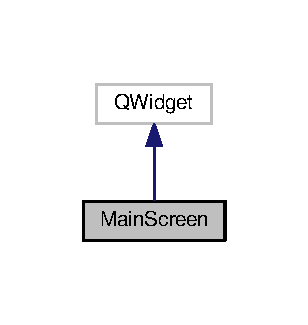
\includegraphics[width=148pt]{class_main_screen__inherit__graph}
\end{center}
\end{figure}


Collaboration diagram for Main\+Screen\+:
\nopagebreak
\begin{figure}[H]
\begin{center}
\leavevmode
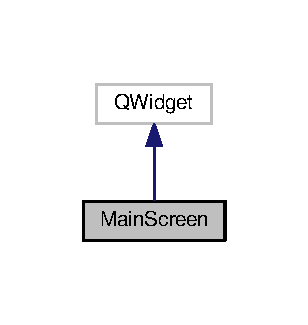
\includegraphics[width=148pt]{class_main_screen__coll__graph}
\end{center}
\end{figure}
\subsection*{Public Slots}
\begin{DoxyCompactItemize}
\item 
void {\bfseries play\+\_\+1} ()\hypertarget{class_main_screen_a8803ff60a438d7fdc64a58dcbd10ee84}{}\label{class_main_screen_a8803ff60a438d7fdc64a58dcbd10ee84}

\item 
void {\bfseries play\+\_\+2} ()\hypertarget{class_main_screen_afcd44fd9e2f02c928b97a2d3c61bb8b0}{}\label{class_main_screen_afcd44fd9e2f02c928b97a2d3c61bb8b0}

\end{DoxyCompactItemize}
\subsection*{Public Member Functions}
\begin{DoxyCompactItemize}
\item 
{\bfseries Main\+Screen} (Q\+Widget $\ast$parent=0)\hypertarget{class_main_screen_a1d65d91f556ec2d850fa7d5b4f7d2d88}{}\label{class_main_screen_a1d65d91f556ec2d850fa7d5b4f7d2d88}

\item 
void {\bfseries play} (const int mode)\hypertarget{class_main_screen_a9a9d7a411606f74f54767edf79ac2408}{}\label{class_main_screen_a9a9d7a411606f74f54767edf79ac2408}

\end{DoxyCompactItemize}


\subsection{Detailed Description}
The \hyperlink{class_main_screen}{Main\+Screen} class represents the startup screen. 

The documentation for this class was generated from the following files\+:\begin{DoxyCompactItemize}
\item 
/home/netsurf/buildspeed/c/src/Main\+Screen.\+h\item 
/home/netsurf/buildspeed/c/src/Main\+Screen.\+cpp\end{DoxyCompactItemize}

\hypertarget{class_player}{}\section{Player Class Reference}
\label{class_player}\index{Player@{Player}}


The \hyperlink{class_player}{Player} class represents the generic player.  




{\ttfamily \#include $<$Player.\+h$>$}



Inheritance diagram for Player\+:\nopagebreak
\begin{figure}[H]
\begin{center}
\leavevmode
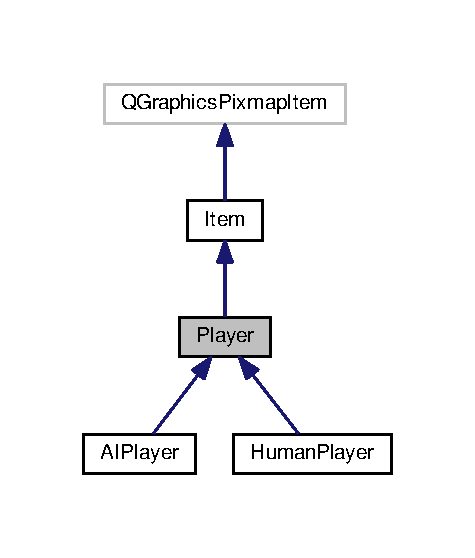
\includegraphics[width=228pt]{class_player__inherit__graph}
\end{center}
\end{figure}


Collaboration diagram for Player\+:\nopagebreak
\begin{figure}[H]
\begin{center}
\leavevmode
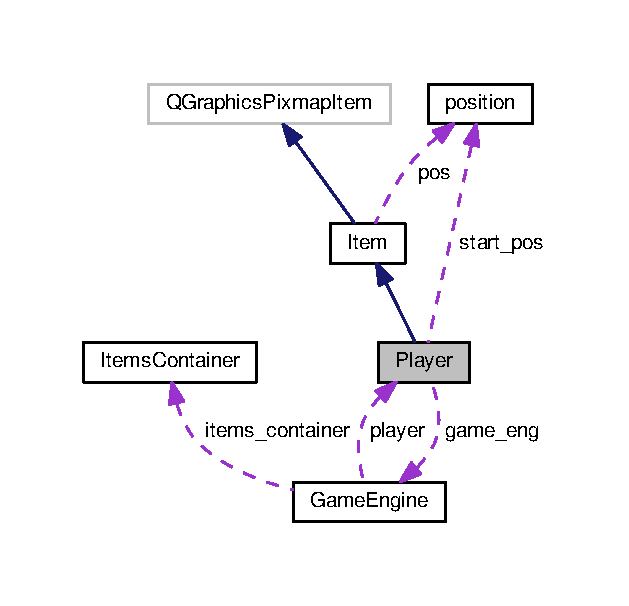
\includegraphics[width=302pt]{class_player__coll__graph}
\end{center}
\end{figure}
\subsection*{Public Member Functions}
\begin{DoxyCompactItemize}
\item 
{\bfseries Player} (\hyperlink{class_game_engine}{Game\+Engine} $\ast$game\+\_\+eng\+\_\+)\hypertarget{class_player_aecff22f81d0d3093d42be398456bbe62}{}\label{class_player_aecff22f81d0d3093d42be398456bbe62}

\item 
void {\bfseries Add\+Score} (const float delta)\hypertarget{class_player_a3e473c9e5749501cc42dbdae5b77d0f2}{}\label{class_player_a3e473c9e5749501cc42dbdae5b77d0f2}

\item 
float {\bfseries Get\+Score} () const \hypertarget{class_player_ac8d63e7ecc7b640d6710462bbc5715d4}{}\label{class_player_ac8d63e7ecc7b640d6710462bbc5715d4}

\item 
\hyperlink{structposition}{position} \hyperlink{class_player_a15005501b35a90791448552245581060}{Get\+Start\+Pos} () const 
\item 
bool \hyperlink{class_player_a68f6b86fc2420f0ee45024e44929ba15}{Can\+Move} () const 
\item 
int {\bfseries Get\+Moves} () const \hypertarget{class_player_a4a9f3ee2deff72685459f606fe640c1d}{}\label{class_player_a4a9f3ee2deff72685459f606fe640c1d}

\item 
bool \hyperlink{class_player_af92895e18f19034043f8274a069afde6}{Move\+In\+Direction} (const int dir)
\begin{DoxyCompactList}\small\item\em moves the player \end{DoxyCompactList}\item 
virtual void {\bfseries Play} ()=0\hypertarget{class_player_aeef5c9637e474dd73ea27e9ffc583dcd}{}\label{class_player_aeef5c9637e474dd73ea27e9ffc583dcd}

\end{DoxyCompactItemize}
\subsection*{Protected Attributes}
\begin{DoxyCompactItemize}
\item 
\hyperlink{structposition}{position} {\bfseries start\+\_\+pos}\hypertarget{class_player_ac150491aec2a800cc12d588f98744b88}{}\label{class_player_ac150491aec2a800cc12d588f98744b88}

\item 
float {\bfseries score}\hypertarget{class_player_aef5032df427b2e15b74477dabc045385}{}\label{class_player_aef5032df427b2e15b74477dabc045385}

\item 
int {\bfseries moves}\hypertarget{class_player_a48886d1a3e0e9093c9ca28dbfec08c38}{}\label{class_player_a48886d1a3e0e9093c9ca28dbfec08c38}

\item 
\hyperlink{class_game_engine}{Game\+Engine} $\ast$ {\bfseries game\+\_\+eng}\hypertarget{class_player_a772e6dd910b610292f7d014a4dfef94a}{}\label{class_player_a772e6dd910b610292f7d014a4dfef94a}

\end{DoxyCompactItemize}
\subsection*{Additional Inherited Members}


\subsection{Detailed Description}
The \hyperlink{class_player}{Player} class represents the generic player. 

It is responsible for moving the character on the grid, receiving score updates, updating tooltips. 

\subsection{Member Function Documentation}
\index{Player@{Player}!Can\+Move@{Can\+Move}}
\index{Can\+Move@{Can\+Move}!Player@{Player}}
\subsubsection[{\texorpdfstring{Can\+Move() const }{CanMove() const }}]{\setlength{\rightskip}{0pt plus 5cm}bool Player\+::\+Can\+Move (
\begin{DoxyParamCaption}
{}
\end{DoxyParamCaption}
) const\hspace{0.3cm}{\ttfamily [inline]}}\hypertarget{class_player_a68f6b86fc2420f0ee45024e44929ba15}{}\label{class_player_a68f6b86fc2420f0ee45024e44929ba15}
\begin{DoxyReturn}{Returns}
true if the player still has moves to do 
\end{DoxyReturn}
\index{Player@{Player}!Get\+Start\+Pos@{Get\+Start\+Pos}}
\index{Get\+Start\+Pos@{Get\+Start\+Pos}!Player@{Player}}
\subsubsection[{\texorpdfstring{Get\+Start\+Pos() const }{GetStartPos() const }}]{\setlength{\rightskip}{0pt plus 5cm}{\bf position} Player\+::\+Get\+Start\+Pos (
\begin{DoxyParamCaption}
{}
\end{DoxyParamCaption}
) const\hspace{0.3cm}{\ttfamily [inline]}}\hypertarget{class_player_a15005501b35a90791448552245581060}{}\label{class_player_a15005501b35a90791448552245581060}
\begin{DoxyReturn}{Returns}
initial player position 
\end{DoxyReturn}
\index{Player@{Player}!Move\+In\+Direction@{Move\+In\+Direction}}
\index{Move\+In\+Direction@{Move\+In\+Direction}!Player@{Player}}
\subsubsection[{\texorpdfstring{Move\+In\+Direction(const int dir)}{MoveInDirection(const int dir)}}]{\setlength{\rightskip}{0pt plus 5cm}bool Player\+::\+Move\+In\+Direction (
\begin{DoxyParamCaption}
\item[{const int}]{dir}
\end{DoxyParamCaption}
)}\hypertarget{class_player_af92895e18f19034043f8274a069afde6}{}\label{class_player_af92895e18f19034043f8274a069afde6}


moves the player 


\begin{DoxyParams}{Parameters}
{\em dir} & is an integer between 0 and 3 (0 -\/ up, 1 -\/ down, 2 -\/ left, 3 -\/ right) \\
\hline
\end{DoxyParams}
\begin{DoxyReturn}{Returns}
true if the move succedeed 
\end{DoxyReturn}


The documentation for this class was generated from the following files\+:\begin{DoxyCompactItemize}
\item 
/home/netsurf/buildspeed/c/src/Player.\+h\item 
/home/netsurf/buildspeed/c/src/Player.\+cpp\end{DoxyCompactItemize}

\hypertarget{structposition}{}\section{position Class Reference}
\label{structposition}\index{position@{position}}


Represents a pair of coordinates on the grid.  




{\ttfamily \#include $<$Item.\+h$>$}

\subsection*{Public Attributes}
\begin{DoxyCompactItemize}
\item 
int {\bfseries x}\hypertarget{structposition_aad0117268685890818989a6c0112ab8a}{}\label{structposition_aad0117268685890818989a6c0112ab8a}

\item 
int {\bfseries y}\hypertarget{structposition_ab7163210f8aa5e8dc68ef434a315792c}{}\label{structposition_ab7163210f8aa5e8dc68ef434a315792c}

\end{DoxyCompactItemize}


\subsection{Detailed Description}
Represents a pair of coordinates on the grid. 

The documentation for this class was generated from the following file\+:\begin{DoxyCompactItemize}
\item 
/home/netsurf/buildspeed/c/src/Item.\+h\end{DoxyCompactItemize}

\hypertarget{class_text_item}{}\section{Text\+Item Class Reference}
\label{class_text_item}\index{Text\+Item@{Text\+Item}}


Inheritance diagram for Text\+Item\+:\nopagebreak
\begin{figure}[H]
\begin{center}
\leavevmode
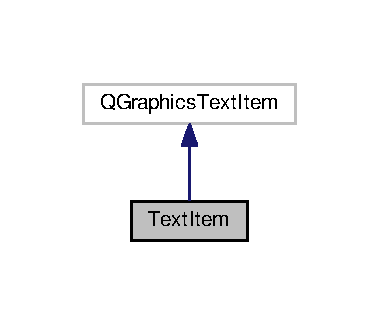
\includegraphics[width=182pt]{class_text_item__inherit__graph}
\end{center}
\end{figure}


Collaboration diagram for Text\+Item\+:\nopagebreak
\begin{figure}[H]
\begin{center}
\leavevmode
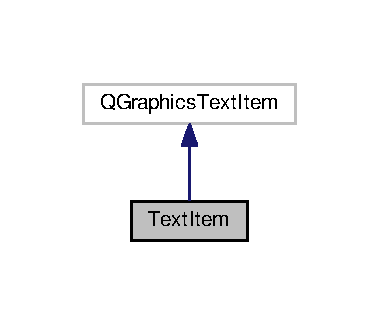
\includegraphics[width=182pt]{class_text_item__coll__graph}
\end{center}
\end{figure}
\subsection*{Public Member Functions}
\begin{DoxyCompactItemize}
\item 
\hyperlink{class_text_item_a6e8b0642b2f4d3f6604728916d00162f}{Text\+Item} (const Q\+String \&text, const int x\+\_\+pos, const int y\+\_\+pos, const Q\+Color bgcolor\+\_\+=B\+A\+C\+K\+G\+R\+O\+U\+N\+D\+\_\+\+C\+O\+L\+OR)\hypertarget{class_text_item_a6e8b0642b2f4d3f6604728916d00162f}{}\label{class_text_item_a6e8b0642b2f4d3f6604728916d00162f}

\begin{DoxyCompactList}\small\item\em constructs a new \hyperlink{class_text_item}{Text\+Item} \end{DoxyCompactList}\item 
virtual Q\+RectF {\bfseries bounding\+Rect} (void) const \hypertarget{class_text_item_a831152f70253ef126712c361cefa01a8}{}\label{class_text_item_a831152f70253ef126712c361cefa01a8}

\item 
virtual void {\bfseries paint} (Q\+Painter $\ast$painter, const Q\+Style\+Option\+Graphics\+Item $\ast$option, Q\+Widget $\ast$widget)\hypertarget{class_text_item_ad453e5bac5a30a89a7c72987b90a1851}{}\label{class_text_item_ad453e5bac5a30a89a7c72987b90a1851}

\item 
virtual Q\+Painter\+Path {\bfseries shape} (void) const \hypertarget{class_text_item_a1b1dca54025a2d9550516f4fd28d4817}{}\label{class_text_item_a1b1dca54025a2d9550516f4fd28d4817}

\item 
Q\+SizeF \hyperlink{class_text_item_a4b0b6f4315c82096ea88690b6936ddb7}{get\+Size} (void) const \hypertarget{class_text_item_a4b0b6f4315c82096ea88690b6936ddb7}{}\label{class_text_item_a4b0b6f4315c82096ea88690b6936ddb7}

\begin{DoxyCompactList}\small\item\em gets size of \hyperlink{class_text_item}{Text\+Item} \end{DoxyCompactList}\item 
void \hyperlink{class_text_item_ac0971ebbb2d234e7da58acbf11ba4a60}{place\+It} (const int x\+\_\+pos, const int y\+\_\+pos)
\begin{DoxyCompactList}\small\item\em sets position of \hyperlink{class_text_item}{Text\+Item} \end{DoxyCompactList}\item 
void \hyperlink{class_text_item_a785f645633f00591d7a33d7f54f72705}{Set\+Value} (const float v)
\begin{DoxyCompactList}\small\item\em stores a numeric value (custom data) along with the \hyperlink{class_text_item}{Text\+Item} \end{DoxyCompactList}\item 
float \hyperlink{class_text_item_ad1824d69e26bd8d7414c1ab6f9a7ed12}{Get\+Value} ()
\begin{DoxyCompactList}\small\item\em gets the numeric value associated with the \hyperlink{class_text_item}{Text\+Item} \end{DoxyCompactList}\end{DoxyCompactItemize}
\subsection*{Protected Attributes}
\begin{DoxyCompactItemize}
\item 
Q\+Color {\bfseries bgcolor}\hypertarget{class_text_item_ad04d01ec588c0c9afa52719cd57cee9e}{}\label{class_text_item_ad04d01ec588c0c9afa52719cd57cee9e}

\item 
float {\bfseries numeric\+\_\+value}\hypertarget{class_text_item_a2310d84d779d095293e504e5c6e2d5ee}{}\label{class_text_item_a2310d84d779d095293e504e5c6e2d5ee}

\end{DoxyCompactItemize}
\subsection*{Static Protected Attributes}
\begin{DoxyCompactItemize}
\item 
static const Q\+Color {\bfseries B\+A\+C\+K\+G\+R\+O\+U\+N\+D\+\_\+\+C\+O\+L\+OR}\hypertarget{class_text_item_a9fa0c74b67dc2e84224d775b5743bdad}{}\label{class_text_item_a9fa0c74b67dc2e84224d775b5743bdad}

\item 
static const qreal {\bfseries M\+A\+R\+G\+IN} = 5\hypertarget{class_text_item_a38fa3b31d77c4972a221afdb41f49f0b}{}\label{class_text_item_a38fa3b31d77c4972a221afdb41f49f0b}

\item 
static const qreal {\bfseries B\+O\+R\+D\+E\+R\+\_\+\+W\+I\+D\+TH} = 1\hypertarget{class_text_item_a951a7e90877fd1c0cb8a97235f0655aa}{}\label{class_text_item_a951a7e90877fd1c0cb8a97235f0655aa}

\item 
static const Q\+Color {\bfseries B\+O\+R\+D\+E\+R\+\_\+\+C\+O\+L\+OR}\hypertarget{class_text_item_a702356977c6e5620dc11694f634fcc27}{}\label{class_text_item_a702356977c6e5620dc11694f634fcc27}

\end{DoxyCompactItemize}


\subsection{Member Function Documentation}
\index{Text\+Item@{Text\+Item}!Get\+Value@{Get\+Value}}
\index{Get\+Value@{Get\+Value}!Text\+Item@{Text\+Item}}
\subsubsection[{\texorpdfstring{Get\+Value()}{GetValue()}}]{\setlength{\rightskip}{0pt plus 5cm}float Text\+Item\+::\+Get\+Value (
\begin{DoxyParamCaption}
{}
\end{DoxyParamCaption}
)\hspace{0.3cm}{\ttfamily [inline]}}\hypertarget{class_text_item_ad1824d69e26bd8d7414c1ab6f9a7ed12}{}\label{class_text_item_ad1824d69e26bd8d7414c1ab6f9a7ed12}


gets the numeric value associated with the \hyperlink{class_text_item}{Text\+Item} 

\begin{DoxyReturn}{Returns}
float value 
\end{DoxyReturn}
\index{Text\+Item@{Text\+Item}!place\+It@{place\+It}}
\index{place\+It@{place\+It}!Text\+Item@{Text\+Item}}
\subsubsection[{\texorpdfstring{place\+It(const int x\+\_\+pos, const int y\+\_\+pos)}{placeIt(const int x_pos, const int y_pos)}}]{\setlength{\rightskip}{0pt plus 5cm}void Text\+Item\+::place\+It (
\begin{DoxyParamCaption}
\item[{const int}]{x\+\_\+pos, }
\item[{const int}]{y\+\_\+pos}
\end{DoxyParamCaption}
)}\hypertarget{class_text_item_ac0971ebbb2d234e7da58acbf11ba4a60}{}\label{class_text_item_ac0971ebbb2d234e7da58acbf11ba4a60}


sets position of \hyperlink{class_text_item}{Text\+Item} 


\begin{DoxyParams}{Parameters}
{\em x,y} & integer coordinates \\
\hline
\end{DoxyParams}
\index{Text\+Item@{Text\+Item}!Set\+Value@{Set\+Value}}
\index{Set\+Value@{Set\+Value}!Text\+Item@{Text\+Item}}
\subsubsection[{\texorpdfstring{Set\+Value(const float v)}{SetValue(const float v)}}]{\setlength{\rightskip}{0pt plus 5cm}void Text\+Item\+::\+Set\+Value (
\begin{DoxyParamCaption}
\item[{const float}]{v}
\end{DoxyParamCaption}
)\hspace{0.3cm}{\ttfamily [inline]}}\hypertarget{class_text_item_a785f645633f00591d7a33d7f54f72705}{}\label{class_text_item_a785f645633f00591d7a33d7f54f72705}


stores a numeric value (custom data) along with the \hyperlink{class_text_item}{Text\+Item} 


\begin{DoxyParams}{Parameters}
{\em float} & value \\
\hline
\end{DoxyParams}


The documentation for this class was generated from the following files\+:\begin{DoxyCompactItemize}
\item 
/home/netsurf/buildspeed/c/src/Text\+Item.\+h\item 
/home/netsurf/buildspeed/c/src/Text\+Item.\+cpp\end{DoxyCompactItemize}

%--- End generated contents ---

% Index
\backmatter
\newpage
\phantomsection
\clearemptydoublepage
\addcontentsline{toc}{chapter}{Index}
\printindex

\end{document}
